% Provenance (never printed): see sources/outline_sources.md (Year 3: Gibbs
% energy and the phase rule in rocks, chemical potential recalled from the
% chemistry book; ternary diagrams; pseudosections, principle). Brief:
% sources/book5/BRIEFS.md, ch. 11. Curves from figdata/bachelor-3/
% gasp_tables.py, schreinemakers.py and regular_solution.py. Exercise and
% problem values in the Book 5 scratch calculator calc/ch11.py.
\chapter{Thermodynamica van gesteenten}\label{ch:b3:petrological-thermodynamics}

Een granaat van enkele millimeter doorsnede groeide zone na zone terwijl zijn schist
begraven en verhit werd. Zijn rand legt in zijn calcium-, ijzer- en magnesiumgehalte
nog vast het laatste evenwicht dat hij bereikte met de biotiet en plagioklaas eromheen.
Boek~4 zette zulke samenstellingen met twee gekalibreerde vergelijkingen om in een
temperatuur en een druk. Dit hoofdstuk opent die doos: waar de vergelijkingen vandaan
komen, hoe ver tabellen met gemeten enthalpieën en entropieën betrouwbaar zijn, hoeveel
mineralen een gesteente kan bevatten, hoe vaste oplossingen mengen en ontmengen, en
hoe een computer een bulksamenstelling omzet in een kaart van de assemblages
die hij moet tonen.

\begin{recall}
De Gibbs-energie, de chemische potentiaal, de activiteit en de
evenwichtsconstante, de variantie en de fasenregel, de mengbaarheidslacune en de
hefboomregel staan in de universitaire delen van de scheikundeboeken. De univariante
reactie, haar Clapeyronhelling $\Delta_rS/\Delta_rV$, het invariante punt en het
aluminosilicaatdiagram berekend uit tabellen staan in Boek~4, in het hoofdstuk over
metamorfe facies; de geothermometer en geobarometer, de
granaat--biotiet-uitwisselingsthermometer en de GASP-barometer, in het hoofdstuk over
P--T--t-paden; ternaire diagrammen en de cotectische lijn, in het hoofdstuk over magma's.
Een vaste oplossing en haar eindleden staan in Boek~3, in het hoofdstuk over
mineralen.
\end{recall}

\section{Evenwicht uit tabellen}\label{sec:b3:petrological-thermodynamics:tables}

Voor een reactie tussen mineralen van vaste samenstelling is evenwicht bij de
temperatuur $T$ en druk $P$ gegeven door $\Delta_rG(T, P) = 0$. Tabellen geven bij
\qty{298.15}{K} en \qty{1}{bar} de vormingsenthalpie, de entropie en het molair
volume van elk mineraal, en daarboven de warmtecapaciteit $C_p(T)$. Boek~4 nam
$\Delta_rH$, $\Delta_rS$ en $\Delta_rV$ als constanten. Het algemene resultaat
luidt als volgt.

\begin{theorem}[Gibbs-energie van een reactie bij $T$ en $P$]\label{thm:b3:petrological-thermodynamics:dg}
Laat een reactie bij $T_0 = \qty{298.15}{K}$ en \qty{1}{bar} de enthalpie
$\Delta_rH^\circ$ en entropie $\Delta_rS^\circ$ hebben, de verandering van de
warmtecapaciteit $\Delta_rC_p(T)$ en, onder de vaste stoffen, een volumeverandering
$\Delta_rV$ die onafhankelijk is van $T$ en $P$. Dan geldt
\[
  \Delta_rG(T, P) = \Delta_rH^\circ + \int_{T_0}^{T}\Delta_rC_p\,\mathrm dT
  - T\Bigl(\Delta_rS^\circ + \int_{T_0}^{T}\frac{\Delta_rC_p}{T}\,\mathrm dT\Bigr)
  + (P - 1)\,\Delta_rV ,
\]
en de evenwichtslijn is $P = 1 - \Delta_rG(T, 1)/\Delta_rV$.
\end{theorem}

\begin{proof}
Bij \qty{1}{bar} geldt $(\partial\Delta_rH/\partial T)_P = \Delta_rC_p$ en
$(\partial\Delta_rS/\partial T)_P = \Delta_rC_p/T$; integreren vanaf $T_0$
geeft $\Delta_rH(T)$ en $\Delta_rS(T)$, en $\Delta_rG = \Delta_rH -
T\Delta_rS$. Bij vaste $T$ geldt $(\partial\Delta_rG/\partial P)_T = \Delta_rV$,
constant volgens de veronderstelling; integreren van 1 tot $P$ levert $(P - 1)\Delta_rV$ op.
Het stellen van $\Delta_rG(T, P) = 0$ levert de lijn op.
\end{proof}

De twee integralen heffen elkaar gedeeltelijk op: hun som is $\int_{T_0}^T\Delta_rC_p(1 -
T/T')\,\mathrm dT'$, waarin de factor $1 - T/T'$ negatief en klein is wanneer
$T'$ dicht bij $T$ ligt. Onder de vaste stoffen is $\Delta_rC_p$ zelf klein,
omdat de warmtecapaciteit van een mineraal vrijwel gelijk is aan de som van die van
zijn oxiden. De benadering van constante eigenschappen is daarom goed, en de
tabellen geven aan hoe goed. Voor de GASP-reactie,
\[
  \ce{3 CaAl2Si2O8 <=> Ca3Al2Si3O12 + 2 Al2SiO5 + SiO2},
\]
geeft de samenvattende tabel $\Delta_rH^\circ = \qty{-36.3}{kJ}$,
$\Delta_rS^\circ = \qty{-130.7}{J.K^{-1}}$ en $\Delta_rV =
\qty{-6.61}{J.bar^{-1}}$, dus een lijn met helling \qty{19.8}{bar/K}; de
hogetemperatuurtabellen, die de warmtecapaciteiten bevatten, geven
$\Delta_rG$ bij elke \qty{100}{K}, en de twee lijnen verschillen minder dan
\qty{0.12}{kbar} tot \qty{1200}{K} (de figuur hieronder).
% ledger: rh95:gasp-298, rh95:gasp-ht

De experimenten komen niet even goed overeen. Omgekeerd in een zuiger-cilinderpers bij
900 tot \qty{1250}{\celsius} ligt de reactie \qty{0.9}{kbar} hoger dan de
tabellen bij \qty{627}{\celsius} en \qty{1.9}{kbar} hoger bij
\qty{927}{\celsius}. Met $\Delta_rV = \qty{-6.61}{J.bar^{-1}}$ komt
\qty{1.9}{kbar} overeen met een fout van \qty{12.6}{kJ} in $\Delta_rH$; de
onzekerheden van de vier vormingsenthalpieën, \qty{3.2}{kJ} voor grossulaar,
\qty{2.0}{kJ} voor anorthiet en kyaniet, \qty{1.0}{kJ} voor kwarts, tellen op
tot ongeveer \qty{8}{kJ} in $\Delta_rH$. Calorimetrie legt elk mineraal vast op
enkele kilojoules; een reactie tussen grote formule-eenheden vermenigvuldigt deze
fouten en deelt ze door een kleine volumeverandering.
% ledger: rh95:gasp-298, kn88:gasp

\begin{definition}[Intern consistente thermodynamische dataset]\label{def:b3:petrological-thermodynamics:dataset}
Een \emph{intern consistente thermodynamische dataset}\index{intern consistente thermodynamische dataset}
is een tabel met de standaardeigenschappen van veel mineralen en vloeistoffen
(vormingsenthalpie, entropie, volume, warmtecapaciteit, thermische uitzetting en
compressibiliteit), gezamenlijk aangepast binnen de onzekerheden van de calorimetrie,
zodat elk daarmee berekend evenwicht door de omgekeerde experimenten
loopt waarop hij is gefit.
\end{definition}

Zo'n dataset wordt één keer gefit, met gewogen kleinste kwadraten of met lineaire
programmering over alle brackets tegelijk, en daarna gebruikt voor elke reactie tussen
zijn mineralen, ook voor reacties die nooit in het laboratorium zijn bestudeerd.
De getallen zijn geen onafhankelijke metingen: één enthalpie kan met een kilojoule
worden verschoven om een reactie waarin hij meedoet te laten kloppen. Waarden uit
verschillende datasets mogen nooit worden gemengd.

\begin{omfigure}
\begin{tikzpicture}
\begin{axis}[omrecord, width=0.78\linewidth, height=0.5\linewidth,
  xlabel={temperatuur (\unit{\celsius})}, ylabel={druk (\unit{kbar})},
  xmin=400, xmax=1300, ymin=0, ymax=30, legend style={font=\scriptsize,
  at={(0.03,0.97)}, anchor=north west, legend cell align=left}]
% computed in figdata/bachelor-3/gasp_tables.py
\fill[omLithLime!60] (axis cs:900,19) rectangle (axis cs:1250,28);
\addplot[red!70!black, very thick] table[x=tc, y=p_kn88] {figdata/out/bachelor-3-gasp_tables-lines.dat};
\addlegendentry{experiment (eindleden)}
\addplot[omDef, thick, densely dashed] table[x=tc, y=p_const] {figdata/out/bachelor-3-gasp_tables-lines.dat};
\addlegendentry{tabellen, constante $\Delta_rH$, $\Delta_rS$}
\addplot[omDef, only marks, mark=*, mark size=1.8pt] table[x=tc, y=p_table] {figdata/out/bachelor-3-gasp_tables-tables.dat};
\addlegendentry{tabellen, met warmtecapaciteiten}
\node[font=\scriptsize, align=center] at (axis cs:1075,26.3) {omgekeerde\\experimenten};
\node[font=\scriptsize] at (axis cs:560,4) {anorthiet};
\node[font=\scriptsize, align=center] at (axis cs:560,17) {grossulaar + kyaniet\\+ kwarts};
\end{axis}
\end{tikzpicture}

\par\smallskip{\small De eindlid-GASP-reactie, 3 anorthiet = grossulaar +
2 kyaniet + kwarts, berekend uit de calorimetrische tabellen met constante
eigenschappen (gestreept) en met de warmtecapaciteiten (stippen), en de lijn die
is gefit aan omgekeerde experimenten in het gearceerde gebied (rood, onder
\qty{900}{\celsius} geëxtrapoleerd).}\label{fig:b3:petrological-thermodynamics:gasp}
\end{omfigure}
% ledger: rh95:gasp-298, rh95:gasp-ht, kn88:gasp

\section{De fasenregel in gesteenten}\label{sec:b3:petrological-thermodynamics:phase-rule}

De fasenregel van de scheikunde geeft de variantie $F = c - p + 2$ van een systeem van
$c$ componenten in $p$ fasen. Een gesteente is zo'n systeem, en zijn mineralen tonen
in welk deel van het druk--temperatuurvlak het in evenwicht was.

\begin{proposition}[Mineralogische fasenregel]\label{prop:b3:petrological-thermodynamics:goldschmidt}
Een gesteente dat in evenwicht is gekomen bij een druk en temperatuur die vrij zijn gekozen
binnen een gebied van het druk--temperatuurvlak, bevat hooguit zoveel fasen als het
componenten heeft: $p \le c$. Dit is de
\emph{mineralogische fasenregel}\index{mineralogische fasenregel}.
\end{proposition}

\begin{proof}
De fasenregel geeft $F = c - p + 2$ onafhankelijke intensieve variabelen. Als de
druk en temperatuur beide kunnen variëren zonder de assemblage te veranderen, zijn er twee
vrij: $F \ge 2$, dus $p \le c$. Een gesteente met $p = c + 1$ fasen ligt
op een univariante lijn; bij $p = c + 2$ op een invariant punt; geen van beide is
waarschijnlijk voor een willekeurig gekozen gesteente.
\end{proof}

Een gesteente dat de regel breekt, is ofwel in evenwicht geweest op een reactielijn, wat de
texturen kunnen tonen, of heeft nooit als geheel evenwicht bereikt: coronatexturen,
gezoneerde mineralen en relictkorrels zijn gangbare redenen. Het tellen van componenten
vraagt zorg. Een component die alleen in één fase van vaste samenstelling voorkomt, zoals
zirkoon, kan samen met die fase worden weggelaten; een component die door een extern
reservoir wordt vastgelegd, zoals water wanneer een vloeistof door het gesteente stroomt, telt
niet als vrij, omdat de chemische potentiaal wordt opgelegd.

Rond een invariant punt kruisen de univariante lijnen elkaar niet willekeurig. In een
systeem van $c$ componenten komen $c + 2$ fasen samen in het punt, en $c + 2$
reacties lopen ervandaan, elk geschreven tussen $c + 1$ fasen en genoemd naar de fase die
ze weglaat, tussen haakjes.

\begin{definition}[Schreinemakers-analyse]\label{def:b3:petrological-thermodynamics:schreinemakers}
\emph{Schreinemakers-analyse}\index{Schreinemakers-analyse} is de methode
die de univariante lijnen rond een invariant punt rangschikt aan de hand van de
samenstellingen van de fasen alleen, vóór enige meting van hun
thermodynamische eigenschappen: zij legt de volgorde van de lijnen vast, de zijde van elke
lijn die stabiel is, en de assemblages van elke sector daartussen.
\end{definition}

\begin{method}[Schreinemakers-regels]\label{met:b3:petrological-thermodynamics:schreinemakers}
(1) Schrijf de $c + 2$ reacties, elk zonder één fase. (2) Elke lijn is
stabiel aan één kant van het punt en metastabiel aan de andere. (3) De
metastabiele verlenging van de ($i$)-lijn, die de fase $i$ weglaat, ligt in een
sector waar $i$ stabiel is. (4) Geen sector tussen twee opeenvolgende stabiele lijnen
overspant meer dan \ang{180}. (5) Over een lijn heen zijn de assemblages aan weerszijden
die van de twee zijden van haar reactie. Het vastleggen van één lijn met gegevens
legt daarna de hele bundel vast, tot op een spiegelbeeld na.
\end{method}

Het aluminosilicaat-drievoudig punt van Boek~4 is het eenvoudigste geval,
$c = 1$ en drie lijnen. De figuur hieronder toont een tweecomponentgeval
berekend door in elk punt de Gibbs-energie te minimaliseren.

\begin{omfigure}
\begin{tikzpicture}
\begin{axis}[omrecord, width=0.62\linewidth, height=0.5\linewidth,
  xlabel={temperatuur (\unit{\celsius})}, ylabel={druk (\unit{kbar})},
  xmin=400, xmax=800, ymin=1, ymax=9, grid=none]
% computed in figdata/bachelor-3/schreinemakers.py
\addplot[omDef, very thick] table[x=t, y=p] {figdata/out/bachelor-3-schreinemakers-ray_A_s.dat};
\addplot[omDef, thick, densely dashed] table[x=t, y=p] {figdata/out/bachelor-3-schreinemakers-ray_A_m.dat};
\addplot[omDef, very thick] table[x=t, y=p] {figdata/out/bachelor-3-schreinemakers-ray_B_s.dat};
\addplot[omDef, thick, densely dashed] table[x=t, y=p] {figdata/out/bachelor-3-schreinemakers-ray_B_m.dat};
\addplot[omDef, very thick] table[x=t, y=p] {figdata/out/bachelor-3-schreinemakers-ray_C_s.dat};
\addplot[omDef, thick, densely dashed] table[x=t, y=p] {figdata/out/bachelor-3-schreinemakers-ray_C_m.dat};
\addplot[omDef, very thick] table[x=t, y=p] {figdata/out/bachelor-3-schreinemakers-ray_D_s.dat};
\addplot[omDef, thick, densely dashed] table[x=t, y=p] {figdata/out/bachelor-3-schreinemakers-ray_D_m.dat};
\node[font=\scriptsize, fill=white, inner sep=1pt] at (axis cs:740,7.85) {(A)};
\node[font=\scriptsize, fill=white, inner sep=1pt] at (axis cs:540,8.75) {(C)};
\node[font=\scriptsize, fill=white, inner sep=1pt] at (axis cs:540,1.6) {(B)};
\node[font=\scriptsize, fill=white, inner sep=1pt] at (axis cs:740,2.15) {(D)};
\node[font=\scriptsize, align=center] at (axis cs:592,7.7) {A + B\\B + D};
\node[font=\scriptsize, align=center] at (axis cs:450,5.0) {A + D};
\node[font=\scriptsize, align=center] at (axis cs:592,2.4) {A + C\\C + D};
\node[font=\scriptsize, align=center] at (axis cs:765,5.0) {A + B\\B + C\\C + D};
\end{axis}
\end{tikzpicture}

\par\smallskip{\small Een Schreinemakers-bundel in een tweecomponentsysteem met
vier fasen met samenstellingen A (0), B ($1/3$), C ($2/3$) en D (1),
berekend voor verzonnen eigenschappen: stabiele lijnen doorgetrokken, metastabiele verlengingen
gestreept, en de stabiele paren in elke sector. (D) is A + C = 2B, (A) is B + D =
2C, (C) is 2A + D = 3B en (B) is A + 2D = 3C.}\label{fig:b3:petrological-thermodynamics:schreinemakers}
\end{omfigure}

\section{Vaste oplossingen}\label{sec:b3:petrological-thermodynamics:solutions}

De meeste gesteentevormende mineralen zijn vaste oplossingen, en hun eindleden verschijnen
in reacties via hun activiteiten. Boek~4 nam $a = X^3$ voor
de grossulaar in een granaat en $a = X$ voor de anorthiet in een plagioklaas.
Beide zijn gevallen van één model.

\begin{definition}[Activiteitsmodel met roostermenging]\label{def:b3:petrological-thermodynamics:site-mixing}
In een \emph{activiteitsmodel met roostermenging}\index{activiteitsmodel met roostermenging}, mengen de
ionen van een mineraal willekeurig op elke kristallografische plaats, onafhankelijk
van de andere plaatsen. De ideale activiteit van een eindlid is dan het product,
over de plaatsen, van de fractie van elke plaats die het vult, verheven tot het aantal
zulke plaatsen per formule-eenheid: $a_i = \prod_s X_{s,i}^{\,n_s}$.
\end{definition}

{\sloppy Een granaat $X_3Y_2\ce{Si3O12}$ heeft drie dodecaëdrische plaatsen $X$ voor
\ce{Ca}, \ce{Fe}, \ce{Mg} en \ce{Mn}: $a_{\text{grossulaar}} =
X_{\text{Ca}}^3$. Een granaat met $X_{\text{Ca}} = 0.10$ bevat
\qty{10}{\percent} grossulaar, maar de activiteit ervan is $10^{-3}$. Het ideale
model telt de configuraties; echte oplossingen hebben daarnaast een overmaatse energie,
omdat ionen van verschillende grootte rek in het rooster veroorzaken.\par}

\begin{definition}[Gibbs-energie--samenstellingsdiagram]\label{def:b3:petrological-thermodynamics:gx}
Een \emph{Gibbs-energie--samenstellingsdiagram}\index{Gibbs-energie--samenstellingsdiagram}
zet, bij vaste temperatuur en druk, de molaire Gibbs-energie van
elke fase van een systeem uit tegen de samenstelling. De stabiele assemblage van elke
bulksamenstelling ligt op de onderste convexe omhullende van de krommen: één fase
waar haar kromme op de omhullende ligt, twee fasen aan de uiteinden van een gemeenschappelijke raaklijn.
\end{definition}

\begin{proposition}[Regelmatige oplossing]\label{prop:b3:petrological-thermodynamics:regular}
In een binaire oplossing met één mengplaats per formule-eenheid en de
wisselwerkingsenergie $W$ is de Gibbs-energie van menging
\[
  G_{\text{mix}} = RT\bigl[x\ln x + (1 - x)\ln(1 - x)\bigr] + Wx(1 - x).
\]
Als $W > 0$, is de oplossing stabiel bij elke samenstelling boven $T_c =
W/(2R)$; onder $T_c$ heeft de kromme twee buigpunten en splitsen de samenstellingen
tussen de twee punten van haar gemeenschappelijke raaklijn zich in twee fasen.
\end{proposition}

\begin{proof}
De eerste term is $-T$ maal de configurationele entropie van willekeurige menging;
de tweede is de eenvoudigste overmaatse energie, symmetrisch en nul aan beide uiteinden.
Twee keer differentiëren geeft $G''_{\text{mix}} = RT/[x(1 - x)] - 2W$. Het minimum
over $x$ ligt bij $x = 1/2$, waar het gelijk is aan $4RT - 2W$, wat positief is bij
elke $x$ als $T > W/(2R)$. Onder die waarde is $G''_{\text{mix}} < 0$ op een interval
rond $1/2$: de kromme buigt daar naar beneden, een rechte lijn tussen twee punten
van de kromme ligt eronder, en volgens de definitie hierboven bestaat het gesteente uit
twee fasen.
\end{proof}

\begin{definition}[Solvus, ontmenging]\label{def:b3:petrological-thermodynamics:solvus}
De \emph{solvus}\index{solvus} is de kromme, in het temperatuur--samenstellingsvlak,
die het mengbaarheidsgat van een vaste oplossing begrenst: onder de solvus is een
enkel kristal van tussenliggende samenstelling onstabiel en splitst het zich in twee.
\emph{Ontmenging (mineraal)}\index{ontmenging (mineraal)} is die splitsing
binnen een kristal bij afkoeling: lamellen van de ene samenstelling groeien in een gastheer van de
andere.
\end{definition}

Alkalivelspaten, pyroxenen en amfibolen vertonen ontmengingslamellen,
zichtbaar onder de microscoop of met het blote oog: de perthiet van veel graniet is
een ontmengd alkalivelspaat, een kaliumrijke gastheer met natriumrijke
lamellen. Tussen de \omterm{def:b3:petrological-thermodynamics:solvus}{solvus} en de spinodale kromme, waar $G''_{\text{mix}} = 0$,
moet een kristal eerst de tweede fase laten ontstaan; binnen de spinodale kromme groeit elke kleine
fluctuatie van de samenstelling door diffusie alleen.

\begin{omfigure}
\begin{tikzpicture}
\begin{groupplot}[group style={group size=2 by 1, horizontal sep=1.7cm},
  omrecord, width=0.47\linewidth, height=0.42\linewidth, title style={font=\small},
  legend style={font=\scriptsize, legend cell align=left}]
\nextgroupplot[title={(a) Gibbs-energie van menging}, xlabel={$x$},
  ylabel={$G_{\text{mix}}$ (\unit{kJ.mol^{-1}})}, xmin=0, xmax=1, ymin=-9, ymax=1,
  legend style={at={(0.5,0.03)}, anchor=south}]
% computed in figdata/bachelor-3/regular_solution.py
\addplot[black, thick, densely dotted] table[x=x, y=g1500] {figdata/out/bachelor-3-regular_solution-gx.dat};
\addlegendentry{\qty{1500}{K}}
\addplot[red!70!black, thick, densely dashed] table[x=x, y=g1203] {figdata/out/bachelor-3-regular_solution-gx.dat};
\addlegendentry{$T_c = \qty{1203}{K}$}
\addplot[omDef, thick] table[x=x, y=g0900] {figdata/out/bachelor-3-regular_solution-gx.dat};
\addlegendentry{\qty{900}{K}}
\addplot[omDef, thin, forget plot] coordinates {(0.111,-0.635) (0.889,-0.635)};
\nextgroupplot[title={(b) solvus en een doorsnede bij $X_0 = 0.3$}, xlabel={$x$},
  ylabel={temperatuur (\unit{K})}, xmin=0, xmax=1, ymin=600, ymax=1300,
  legend style={at={(0.5,0.03)}, anchor=south}]
\addplot[omDef, thick] table[x=x, y=t_bin] {figdata/out/bachelor-3-regular_solution-solvus.dat};
\addlegendentry{solvus}
\addplot[black, thick, densely dotted] table[x=x, y=t_spin] {figdata/out/bachelor-3-regular_solution-solvus.dat};
\addlegendentry{spinodale kromme}
\addplot[red!70!black, thick, forget plot] coordinates {(0.3,600) (0.3,1300)};
\addplot[red!70!black, thick, densely dashed] table[x=x2, y=t] {figdata/out/bachelor-3-regular_solution-section.dat};
\addlegendentry{isopleten bij $X_0$}
\addplot[red!70!black, thick, densely dashed, forget plot] table[x=x1, y=t] {figdata/out/bachelor-3-regular_solution-section.dat};
\node[font=\scriptsize] at (axis cs:0.5,1250) {één fase};
\node[font=\scriptsize] at (axis cs:0.5,950) {twee fasen};
\end{groupplot}
\end{tikzpicture}

\par\smallskip{\small Een regelmatige oplossing met $W = \qty{20}{kJ.mol^{-1}}$
(ter illustratie). (a) Gibbs-energie van menging bij drie temperaturen; bij
\qty{900}{K} raakt de gemeenschappelijke raaklijn (dunne lijn) de kromme bij $x = 0.11$
en 0.89. (b) De \omterm{def:b3:petrological-thermodynamics:solvus}{solvus} en de spinodale kromme; een gesteente met bulksamenstelling $X_0 =
0.3$ (verticale rode lijn) is één fase boven \qty{1136}{K} en twee fasen
eronder, waarvan de samenstellingen de \omterm{def:b3:petrological-thermodynamics:solvus}{solvus} volgen (gestippeld).}\label{fig:b3:petrological-thermodynamics:solvus}
\end{omfigure}

\section{Pseudosecties}\label{sec:b3:petrological-thermodynamics:pseudosections}

Paneel (b) van de figuur hierboven is al een kleine \omterm{def:b3:petrological-thermodynamics:pseudosection}{pseudosectie}: voor één
bulksamenstelling geeft het aan welke fasen bij elke temperatuur stabiel zijn, en wat
hun samenstellingen en verhoudingen zijn. Een metamorf gesteente heeft ongeveer tien
componenten en veel vaste oplossingen, maar het principe is hetzelfde.

\begin{definition}[Gibbs-energieminimalisatie]\label{def:b3:petrological-thermodynamics:minimisation}
\emph{Gibbs-energieminimalisatie}\index{Gibbs-energieminimalisatie} zoekt, bij een
gegeven temperatuur en druk, de verzameling fasen, hun samenstellingen en
hun hoeveelheden die de totale Gibbs-energie van een systeem met vaste
bulksamenstelling minimaliseert, onder de voorwaarde dat elke component behouden blijft.
\end{definition}

\begin{definition}[Pseudosectie, isopleet, effectieve bulksamenstelling]\label{def:b3:petrological-thermodynamics:pseudosection}
Een \emph{pseudosectie}\index{pseudosectie} is een fasediagram, meestal in
het druk--temperatuurvlak, berekend voor één vaste bulksamenstelling: het
is verdeeld in velden, elk gelabeld met de assemblage die daar de Gibbs-energie minimaliseert. Een
\emph{isopleet (pseudosectie)}\index{isopleet (pseudosectie)}
is een lijn van een pseudosectie waarlangs een samenstellingsvariabele van één fase, of
de hoeveelheid ervan, constant is. De \emph{effectieve
bulksamenstelling}\index{effectieve bulksamenstelling} is het deel van de
samenstelling van het gesteente dat nog aan het evenwicht deelneemt, nadat de kernen van gezoneerde
kristallen, porfyroblasten die van de matrix zijn afgesloten en andere
geïsoleerde materie zijn verwijderd.
\end{definition}

Een \omterm{def:b3:petrological-thermodynamics:pseudosection}{pseudosectie} toont geen univariante lijnen in de zin van Boek~4:
in een systeem met vaste oplossingen is de grens tussen twee velden de plaats
waar één fase verschijnt of verdwijnt, en de ligging ervan hangt af van de
bulksamenstelling. Een \omterm{def:b3:petrological-thermodynamics:pseudosection}{pseudosectie} aflezen gaat rechtstreeks. De waargenomen assemblage legt een veld vast;
de gemeten samenstelling van een mineraal, bijvoorbeeld het calcium van een granaatrand, kiest
daarbinnen een isopleet; een tweede isopleet, van een ander element of een ander mineraal,
snijdt die bij de druk en de temperatuur van het evenwicht.
Gezoneerde granaten dragen zo een reeks snijpunten, één per zone, langs het traject van het gesteente.
Maar naarmate de granaat groeit, onttrekt zijn kern mangaan en calcium aan het bereik
van de matrix: de \omterm{def:b3:petrological-thermodynamics:pseudosection}{effectieve bulksamenstelling} verandert, en de \omterm{def:b3:petrological-thermodynamics:pseudosection}{pseudosectie}
moet opnieuw worden berekend
voor de latere zones.

\begin{inthelab}[De werkplek van de petroloog]
\begin{minipage}[t]{0.55\linewidth}\vspace{0pt}
De petroloog bestudeert eerst een slijpplaatje onder de polarisatiemicroscoop,
om de assemblage, de texturen en welke korrels samen zijn gegroeid, vast te stellen.
Datzelfde slijpplaatje, bedekt met koolstof, gaat daarna naar een elektronenmicrosonde,
die de samenstelling meet van plekjes van enkele micrometer groot
langs profielen door de granaten. Software die de Gibbs-energie minimaliseert
met een \omterm{def:b3:petrological-thermodynamics:dataset}{intern consistente thermodynamische dataset} en een reeks activiteitsmodellen berekent
een \omterm{def:b3:petrological-thermodynamics:pseudosection}{pseudosectie} voor de bulksamenstelling, gemeten aan een plakje van hetzelfde
gesteente. De isopleten van de gemeten samenstellingen worden erop uitgezet, en waar
ze elkaar snijden, ligt het antwoord. De onzekerheid van de dataset en van de activiteitsmodellen,
niet die van de metingen, beperkt die meestal.
\end{minipage}\hfill
\begin{minipage}[t]{0.42\linewidth}\vspace{0pt}
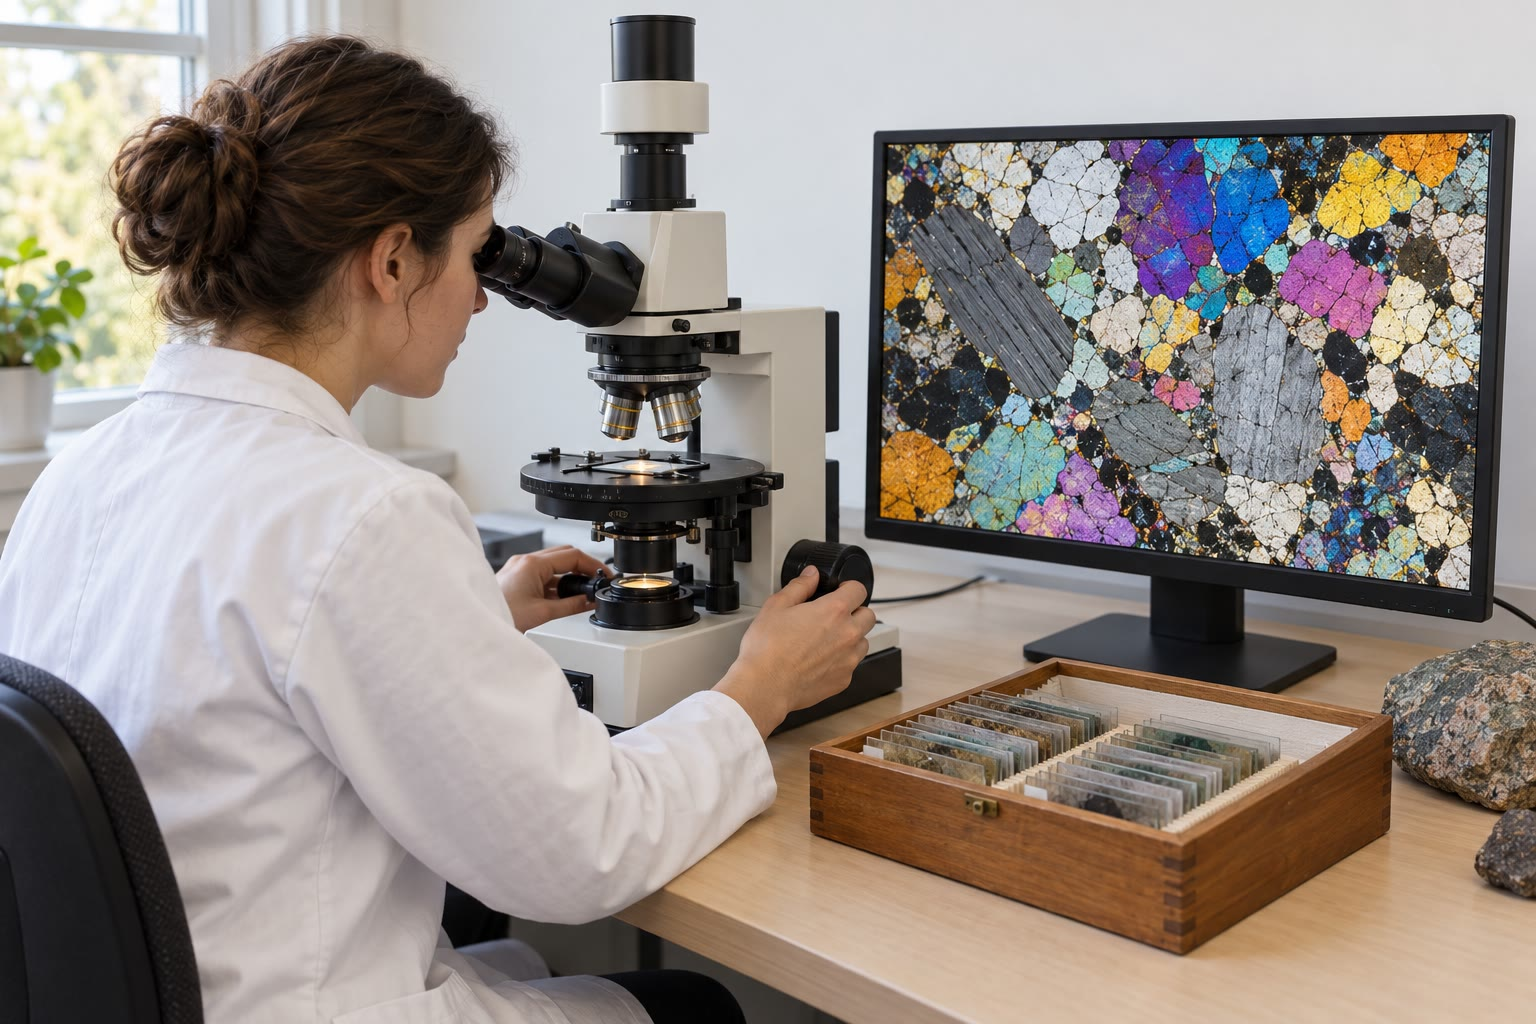
\includegraphics[width=\linewidth]{images/book5/ai/b3-petrology-desk.jpg}

{\scriptsize Een petroloog aan een polarisatiemicroscoop, een doos slijpplaatjes
binnen handbereik en een slijpplaatje in gepolariseerd licht op het scherm
Door AI gegenereerde illustratie.}
\end{minipage}
\end{inthelab}

\section{Oefeningen}

\begin{exercise}[$\star$]\label{exo:b3:petrological-thermodynamics:1}
Uit de tabellen heeft albiet $\Delta_fH^\circ = \qty{-3935.0}{kJ}$, $S^\circ =
\qty{207.4}{J.K^{-1}}$, $V = \qty{100.07}{cm^3}$; jadeïet $-3029.3$, 133.5,
60.40; kwarts $-910.7$, 41.5, 22.69 (per mol). Voor albiet = jadeïet + kwarts,
bereken $\Delta_rH$, $\Delta_rS$, $\Delta_rV$ (in \unit{J.bar^{-1}}), de
Clapeyronhelling en de druk van de lijn bij \qty{600}{\celsius} met
constante eigenschappen.
\end{exercise}
% ledger: rh95:ab-jd-qz

\begin{exercise}[$\star$]\label{exo:b3:petrological-thermodynamics:2}
Een gesteente van het systeem \ce{MgO}--\ce{SiO2} bevat forsteriet, enstatiet en
kwarts. Pas de \omterm{prop:b3:petrological-thermodynamics:goldschmidt}{mineralogische fasenregel} toe. Welke conclusie volgt eruit?
\end{exercise}

\begin{exercise}[$\star$]\label{exo:b3:petrological-thermodynamics:3}
Bereken de ideale activiteiten van grossulaar en pyrop in een granaat met
$X_{\text{Ca}} = 0.20$ en $X_{\text{Mg}} = 0.15$, en van anorthiet in een
plagioklaas met $X_{\text{an}} = 0.40$ (één roosterplaats).
\end{exercise}

\begin{exercise}[$\star$]\label{exo:b3:petrological-thermodynamics:4}
Bereken de kritische temperatuur van een regelmatige oplossing met $W =
\qty{15}{kJ.mol^{-1}}$. Welke $W$ geeft $T_c = \qty{1000}{K}$?
\end{exercise}

\begin{exercise}[$\star\star$]\label{exo:b3:petrological-thermodynamics:5}
Bij \qty{1000}{K} geven de tabellen de Gibbs-energieën van vorming
$-5432.2$ (grossulaar), $-3478.1$ (anorthiet), $-2088.8$ (kyaniet) en $-730.2$
(kwarts), in \unit{kJ.mol^{-1}}. Bereken $\Delta_rG$ van de GASP-reactie bij
\qty{1}{bar} en de evenwichtsdruk ervan, en vergelijk met de experimentele
lijn $P_0 = 22.80\,T - 1093$ (bar, \unit{\celsius}).
\end{exercise}
% ledger: rh95:gasp-ht, kn88:gasp

\begin{exercise}[$\star\star$]\label{exo:b3:petrological-thermodynamics:6}
Voor de regelmatige oplossing uit de figuur ($W = \qty{20}{kJ.mol^{-1}}$), bereken
$G_{\text{mix}}$ bij $x = 0.5$ en \qty{900}{K}, daarna bij de solvusflank $x =
0.111$. Toon aan dat het splitsen van een kristal met samenstelling 0.5 in de twee flanken
de Gibbs-energie verlaagt, en met hoeveel.
\end{exercise}

\begin{exercise}[$\star\star$]\label{exo:b3:petrological-thermodynamics:7}
Hoeveel fasen komen samen in een invariant punt, en hoeveel univariante lijnen
gaan er vanuit het punt uit, in een systeem van drie componenten? In de bundel van de
figuur, controleer dat elk van de vier reacties klopt.
\end{exercise}

\begin{exercise}[$\star\star$]\label{exo:b3:petrological-thermodynamics:8}
Een gesteente met bulksamenstelling $X_0 = 0.3$ in de regelmatige oplossing van de figuur
is afgekoeld tot \qty{900}{K}, waar de solvusflanken 0.111 en 0.889 zijn.
Bereken de hoeveelheid van elke fase.
\end{exercise}

\begin{exercise}[$\star\star$]\label{exo:b3:petrological-thermodynamics:9}
Met de GASP-barometer $P = P_0 + (3RT/6.21)\ln(X_{\text{Ca}}/X_{\text{an}})$
(bar), bereken $\partial P/\partial X_{\text{an}}$ bij \qty{900}{K} en
$X_{\text{an}} = 0.30$. Met hoeveel verschuift de druk, als de waarde van
$X_{\text{an}}$ met 0.01 afwijkt?
\end{exercise}

\begin{exercise}[$\star\star\star$]\label{exo:b3:petrological-thermodynamics:10}
Toon aan dat de spinodaal van een regelmatige oplossing gelijk is aan $x(1 - x) = RT/(2W)$. Bij welke
temperatuur wordt een kristal met samenstelling 0.3 instabiel voor elke kleine
fluctuatie, voor $W = \qty{20}{kJ.mol^{-1}}$? Vergelijk met de temperatuur waarbij
het de \omterm{def:b3:petrological-thermodynamics:solvus}{solvus} bereikt, $T = W(1 - 2x)/[R\ln((1 - x)/x)]$, en verklaar
de kloof.
\end{exercise}

\begin{exercise}[$\star\star\star$]\label{exo:b3:petrological-thermodynamics:11}
Toon aan dat de \omterm{def:b3:petrological-thermodynamics:solvus}{solvus} van een symmetrische regelmatige oplossing voldoet aan $RT\ln[x/(1 -
x)] + W(1 - 2x) = 0$, en dat hij zijn maximum, $T_c = W/(2R)$, bereikt bij $x
= 1/2$.
\end{exercise}

\begin{exercise}[$\star\star\star$]\label{exo:b3:petrological-thermodynamics:12}
Een gesteente bevat \qty{2.0}{wt\percent} \ce{MnO}. Granaatkernen met
\qty{10}{wt\percent} \ce{MnO} vormen \qty{8}{wt\percent} van het gesteente en zijn
afgesloten van de matrix. Bereken het \ce{MnO}-gehalte van de effectieve bulk
samenstelling. Waarom is dat belangrijk voor de \omterm{def:b3:petrological-thermodynamics:pseudosection}{pseudosectie} van de granaatranden?
\end{exercise}

\section{Probleem: het granaat van de Varden-schist}

\begin{problem}[{Weekendprobleem --- de druk en temperatuur van een verzonnen
schist, uit tabellen, de fasenregel, activiteitsmodellen en
thermobarometrie}]
\label{pb:b3:petrological-thermodynamics:1}
% values: calc/ch11.py; gasp_tables.py
De schist van het Varden Hills-basement, ongeveer
\qty{480}{Ma} geleden gemetamorfoseerd, bevat granaat, biotiet, muscoviet, plagioklaas, kyaniet en
kwarts. Aan de rand van een granaat en in de korrels eromheen meet de microsonde:
granaat $X_{\text{Fe}} = 0.74$, $X_{\text{Mg}} = 0.12$, $X_{\text{Ca}} =
0.10$, $X_{\text{Mn}} = 0.04$; biotiet $\ce{Mg}/(\ce{Mg} + \ce{Fe}) = 0.45$;
plagioklaas $X_{\text{an}} = 0.30$. Gebruik de tabellen van dit hoofdstuk voor de
GASP-reactie, de thermometer uit Boek~4
\[
T = \frac{52\,635 + 0.311P}{20.20 - 3R\ln K_D}\quad(T \text{ in K}, P
\text{ in bar}),
\]
en de experimentele barometer $P = 22.80\,t - 1093 + (3RT/6.21)\ln
(X_{\text{Ca}}/X_{\text{an}})$, met $t$ in \unit{\celsius} en $T$ in
kelvin. Neem $R = \qty{8.314}{J.mol^{-1}.K^{-1}}$, een korstdichtheid van
\qty{2800}{kg/m^3} en $g = \qty{9.81}{m/s^2}$.

\medskip\noindent\textbf{Deel I --- De tabellen.}
\begin{enumerate}
  \item Bereken uit de samenvattende tabel $\Delta_rH^\circ$, $\Delta_rS^\circ$
        en $\Delta_rV$ van de GASP-reactie.
  \item Bereken $\Delta_rG$ bij \qty{298.15}{K} en \qty{1}{bar}. Welke kant
        is aan het oppervlak stabiel?
  \item Bereken de eindliddruk bij \qty{900}{K} met constante
        eigenschappen, en de Clapeyronhelling.
  \item De hogetemperatuurtabellen geven $\Delta_rG = \qty{81.5}{kJ}$ bij
        \qty{900}{K} en \qty{119.8}{kJ} bij \qty{1200}{K} (\qty{1}{bar}).
        Bereken de drukken.
  \item Vergelijk met de experimentele lijn bij dezelfde temperaturen.
  \item Welke fout in $\Delta_rH$ zou de kloof bij \qty{1200}{K} verklaren?
        Vergelijk met de gecombineerde onzekerheid van de vier enthalpieën.
  \item Waarom veranderen de warmtecapaciteiten het resultaat zo weinig?
\end{enumerate}

\medskip\noindent\textbf{Deel II --- De fasenregel.}
\begin{enumerate}[resume]
  \item Geef de componenten die nodig zijn om de zes mineralen en een waterig
        fluïdum te beschrijven, en tel de fasen.
  \item Bereken de variantie met de fasenregel en controleer de \omterm{prop:b3:petrological-thermodynamics:goldschmidt}{mineralogische
        fasenregel}.
  \item Een tweede monster bevat kyaniet en sillimaniet naast elkaar. Wat zegt
        dit over de druk en temperatuur?
  \item Water stroomde tijdens de metamorfose door het gesteente. Hoe verandert
        dat de telling?
\end{enumerate}

\medskip\noindent\textbf{Deel III --- Activiteiten en thermobarometrie.}
\begin{enumerate}[resume]
  \item Bereken de ideale activiteiten van grossulaar en anorthiet, en $\ln K$
        van de GASP-reactie in het gesteente.
  \item Bereken $K_D$ van de granaat--biotiet-uitwisseling.
  \item Bereken de temperatuur bij \qty{8}{kbar}.
  \item Bereken de GASP-druk bij die temperatuur.
  \item Itereer naar het snijpunt van de twee vergelijkingen.
  \item Herhaal het snijpunt met de eindlijn uit de tabellen in plaats van
        de experimentele lijn (met $\Delta_rV = \qty{-6.61}{J.bar^{-1}}$).
        Welk resultaat wordt aangehouden, en waarom?
  \item Hoeveel verschuift het resultaat bij een fout van 0.05 in
        $X_{\text{an}}$?
\end{enumerate}

\medskip\noindent\textbf{Deel IV --- De begraving.}
\begin{enumerate}[resume]
  \item Met de constante eigenschappen van Boek~4 heeft kyaniet =
        sillimaniet $\Delta_rH = \qty{7.7}{kJ}$, $\Delta_rS =
        \qty{12.6}{J.K^{-1}}$, $\Delta_rV = \qty{0.571}{J.bar^{-1}}$. Ligt het
        resultaat in het kyanietveld?
  \item Bereken de begravingsdiepte.
  \item De granaatkern heeft $X_{\text{Ca}} = 0.07$ en groeide met plagioklaas
        van dezelfde $X_{\text{an}}$, bij ongeveer dezelfde temperatuur. Is de
        kern dieper of ondieper gevormd dan de rand?
  \item Geef de piekdruk en begravingsdiepte van de Varden-schist.
\end{enumerate}
\end{problem}
